\chapter{Introduction}
\label{chapt:intro}
\chapterPage{
Model-driven engineering methodology and dynamically adaptive systems approach are combined to tackle new challenges brought by systems nowadays. 
After introducing these two software engineering techniques, I give one example of such systems: the Luxembourg smart grid. 
I will also use this example to highlight two of the problematics: uncertainty of data and delays in actions. 
Among the different challenges which are implied by them, I present the global one addressed by the vision defended in this thesis: modeling of temporal and uncertain data. 
This global challenge can be addressed by splitting up in several ones. I present two of them, which are directly tackled by two contributions presented in this thesis.
}

%\section{Introduction}

%% Research questions
\paragraph{Delayed actions}
General research question:
\begin{center}
	\textbf{RQ1}: Do current state of the art solutions allow modeling and reasoning over delayed actions?  
\end{center}

Sub research questions:
\begin{itemize}
	\item \textbf{RQ1.1}: How current approaches model the evolution of the context and/or the evolution of the behavior of systems over time?
	\item \textbf{RQ1.2}: Do these solutions model actions, their circumstances and their effects?
	\item \textbf{RQ1.3}: What are the solutions that enable the reasoning over the evolving context and/or behavior of systems?
\end{itemize}


\paragraph{Uncertainty}

%% Methodology
Snowballing approach~\cite{DBLP:conf/ease/Wohlin14}

\paragraph{Inclusion criteria}
\begin{itemize}
	\item \textbf{IC1}: The paper has been published before the May 31 2019
	\item \textbf{IC2}: The paper is available online and written in English
	\item \textbf{IC3}: The paper describes a modeling approach that abstract the context or behavior of a system.
	\item \textbf{IC4}: The paper describes an approach that enables to reason or navigate through a temporal model.
\end{itemize}

\paragraph{Exclusion criteria}
\begin{itemize}
	\item \textbf{EC1}: The paper has less than 4 pages (short paper).
	\item \textbf{EC2}: The paper presents a work in progress (workshop papers), a poster, vision or doctoral studies.
	\item \textbf{EC3}: The paper describes a secondary study (\eg literature reviews, lessons learned).
	\item \textbf{EC4}: The document has not been published in a venue with a peer-review process. For example, technical and research report or white papers.
	\item \textbf{EC5}: The document is an introduction to the proceedings of a venue or a special issue.
\end{itemize}

However, the references of papers rejected are considered for the snowballing iteration.
%\section{Use case: Luxembourg smart grid}
\label{sec:intro:use-case}

Should contain:
	
	

\section{Context}
Utilities are introducing more and more \gls{ict} in the grid in order to face the new challenges of electricity supply~\cite{farhangi2010path, ipakchi2009grid, DBLP:journals/comsur/FangMXY12}.
These nowadays power grids are referred to as \gls{sg}.

In this document, we focus on the \textbf{\gls{shealing}} capacity of such grids.
A \gls{shealingSyst} can automatically repair any incident, software or hardware, at runtime~\cite{DBLP:journals/computer/KephartC03}.
For example, a smart grid can optimize the power flow to deal with failures of transformers\footnote{Transformers change the voltage in cables.}~\cite{DBLP:journals/comsur/FangMXY12}.
In this way, the incident will impact as few users as possibles, ideally none. 

This healing mechanism can be performed only if the smart grid has a deep understanding of itself and its environment.
To tame their complexity, a common approach in software engineers is to use an \textbf{abstraction} mechanism.
Abstractions provide an illuminating description of systems, their behaviours, or their environment.
For example, Hartmann~\etal \cite{DBLP:conf/smartgridcomm/0001FKTPTR14} provide a class diagram that describes the smart grid topology, when it uses power-line communications\footnote{Data are sent through cables that also distribute electricity.}.

\bigskip

More generally, a \gls{shealing} is a \textbf{\gls{sadapt}}. 
Cheng \etal define \glspl{sadapt} as \textquote{systems that are able to adjust their behaviour in response to their perception of the environment and the system itself}~\cite{DBLP:conf/dagstuhl/ChengLGIMABBBCSDFGGGKKKLMMMPSTTWW09}.
Jeffrey O. Kephart and David M. Chess~\cite{DBLP:journals/computer/KephartC03} laid the groundwork of this approach, based on an IBM white paper~\cite{computing2006architectural}.
Since then, it has been used in different domain~\cite{DBLP:journals/corr/abs-1904-01518} such as cloud infrastructure~\cite{DBLP:conf/icac/JavadiG17, OpenStack:Watcher:Wiki, DBLP:conf/icse/BarnaKFL17} or \gls{cps}~\cite{DBLP:conf/icac/LalandaGC17, DBLP:conf/cbse/FouquetMFBPJ12, DBLP:conf/smartgridsec/0001FKNT14}.

\textbf{\Gls{mde}} uses the abstraction mechanism to facilitate the development of nowadays software~\cite{DBLP:journals/computer/Schmidt06, DBLP:conf/ifm/Kent02, DBLP:series/synthesis/2017Brambilla}.
This methodology can be applied to different stages of software development.
In this thesis, we focus on one of its paradigm: \textbf{\gls{m@rt}}~\cite{DBLP:journals/computer/BlairBF09, DBLP:journals/computer/MorinBJFS09}.
The state of the system or its environment, as well as its behaviour, are reflected in a model, used for analysis.
Developers can use this paradigm to implement \glspl{adptSyst}~\cite{DBLP:journals/computer/MorinBJFS09, DBLP:conf/smartgridsec/0001FKNT14}.

\bigskip

Whereas smart grids introduce more and more automation capacity, human interventions are still required.
First, information gathered by smart grids is therefore not always known with absolute confidence.
Second, smart grids reconfigurations are not immediate, and their effects are not instantaneously measured.
Third, smart grids behaviour is emergent~\cite{zio2011uncertainties}, \ie it cannot be entirely known at design time.

Most fuses are manually open and close by technicians rather than automatically modified.
Then, technicians manually report the modifications done on the grid.
Due to human mistakes, this results in errors.
The grid topology is thus uncertain.
This uncertainty is propagated to the load approximation, used to detect overloads in the grid.
Wrong reconfigurations might be triggered, which could be even worse than if no change would have been applied.

Reconfiguring a smart grid implied to change the power flow.
It is done by connecting or disconnecting specific cables.
That is, opening or closing fuses.
As said before, a technician needs to drive physically to the fuse location to modify its state.
Besides, in the case of the Luxembourg smart grid, meters send energy measurement every 15 mins, non-synchronously.
Between the time a reconfiguration of the smart grid is decided, and the time the effects are measured, a delay of at least 15 mins occurs.
On the other hand, an incident should be detected in the next minutes.
If the adaptation process does not consider this difference of paces, it can cause repeated decisions.

Smart grid behaviour is affected by several factors that cannot be controlled by the grid manager.
One example is the weather condition.
Smart grids rely on an energy production that is distributed over several actors.
For instance, users, who were mainly consumers before, now produce energy by adding solar panels on the roof of their houses.
The production of such energy depends on the weather, and even on the season\footnote{The angle of the sun has an impact on the amount of energy produced by solar panels. This angle varies according to the season.}.
Another example is the increasing adoption of electric vehicles, which de facto drastically increase the consumption of electricity during the night.
Ignoring this characteristic of \gls{adptSyst} may result in suboptimal situations that can be understood with difficulties.
\section{Problem statement}

During our study, we have identified several characteristics of \glspl{adptSyst} that bring challenges to the software engineering research community.
First, information gathered is not always known with absolute confidence.
Second, reconfigurations may not be immediate, and their effects are not instantaneously measured.
Third, system behaviour may be emergent~\cite{zio2011uncertainties}, \ie it cannot be entirely known at design time.
Four, the different sub-parts of the system do not evolve at the same pace.
Five, structure and behaviour of systems have a time dimension.


\subsection{Data are uncertain}
Most fuses are manually open and close by technicians rather than automatically modified.
Then, technicians manually report the modifications done on the grid.
Due to human mistakes, this results in errors.
The grid topology is thus uncertain.
This uncertainty is propagated to the load approximation, used to detect overloads in the grid.
Wrong reconfigurations might be triggered, which could be even worse than if no change would have been applied.

More generally, \textbf{data are, almost by definition, uncertain and developers always work with estimates}~\cite{DBLP:conf/asplos/BornholtMM14, metrology2008evaluation, DBLP:journals/tkde/AggarwalY09}.
The uncertainty may be explained by how data are collected.
We can distinguish three categories: sensors, humans, and results of computations.
Sensors (software or hardware) always estimate the value and have a precision value due to the method of measurement~\cite{metrology2008evaluation, DBLP:conf/asplos/BornholtMM14}.
Humans are error-prone.
And computations can either give an approximation or be based on uncertain data.
This uncertainty is then propagated through all steps until the final result.

For a specific domain, this uncertainty may impact the understanding of the real situation.
For example, the uncertainty of the \gls{cpu} clock is too low to damage the percentage load of the processor.
However, the uncertainty of the \gls{gps} may impact the understanding by, for instance, showing the user on the wrong road (compared to the real one).
\textbf{If the data uncertainty can mislead the understanding of a system behaviour or state, then developers should implement an uncertainty-aware system.}
For \glspl{adptSyst}, this lack of confidence may trigger suboptimal adaptations.


\subsection{Actions have long-term effects}
Reconfiguring a smart grid implied to change the power flow.
It is done by connecting or disconnecting specific cables.
That is, opening or closing fuses.
As said before, technicians need to drive physically to fuse locations to modify their states.
Besides, in the case of the Luxembourg smart grid, meters send energy measurement every 15 mins, non-synchronously.
Between the time a reconfiguration of the smart grid is decided, and the time the effects are measured, a delay of at least 15 mins occurs.
On the other hand, an incident should be detected in the next minutes.
If the adaptation process does not consider this difference of paces, it can cause repeated decisions.

\textbf{Actions are never immediate, take time to be executed, and have long-term effects.}
Through this thesis, we refer to such actions as \glspl{longTermAct}.
In computer science, the definition of "immediate" is specific to a domain.
For example, in graphical user interface, a response time of less than 200 ms is considered as immediate.
However, at while working at the processor level, the execution time of an instruction is measured at the nano seconds scale.

Not considering this delay may lead to sub-optimal decisions.
For example, not considering the delay for the system to handle the migration of a virtual machine may lead to repeat decisions.
We argue that \textbf{developers should take into account this delay if the frequency of the monitoring stage is lower than the time of action effects to be measurable}.

\subsection{Systems may have emergent behaviours}
Smart grid behaviour is affected by several factors that cannot be controlled by the grid manager.
One example is the weather condition.
Smart grids rely on an energy production that is distributed over several actors.
For instance, users, who were mainly consumers before, now produce energy by adding solar panels on the roof of their houses.
The production of such energy depends on the weather, and even on the season\footnote{The angle of the sun has an impact on the amount of energy produced by solar panels. This angle varies according to the season.}.
Another example is the increasing adoption of electric vehicles, which de facto drastically increase the consumption of electricity during the night.
Ignoring this characteristic of \gls{adptSyst} may result in suboptimal situations that can be understood with difficulties.

\textbf{System behaviour may be emergent.}~\cite{zio2011uncertainties}
Different factor can explain this phenomena.
As for \glspl{sg}, systems may evolve in a stochastic and uncertain environment.
Or, some system, like those name ultra-large systems, are so complex that none of the engineer can tame it.
But, groups of engineers will have an understanding of some part of the system.

Despite the complexity, engineers still need to understand how the system is behaving or behaved.
This will help them to optimise the global behaviour or to understand and repair errors.
\textbf{Engineers need tooling support to trace back previous behaviour and or replay them.}


\subsection{Different part of a system evolve at different paces}
Every meters send consumption and production data every 15 mins.
However, this collection is not synchronous.
That is, all meters do not send their data at the same timestamp.
The global system, which receive all data, has not thus a global vision with the same freshness for all the part of the grid.
Electricity data are very volatile: a peak or a drop may happen in less than a minute due to, for instance, the starting or the finishing of a washing machine.
When analysing the data, the process should consider this difference of paces, and estimate the evolution of data.
Otherwise, they will reason over outdated data, which do not reflect the real situation.
This may lead to suboptimal decisions.

\textbf{Different part of the same system may evolve at different paces.}
Some systems are heterogeneous in term of hardware and software.
This diversity results in different evolution or reaction paces.
For example, if some component are working on batteries, they will have a sleep cycle in order to save energy.
Contrary, if some others are running directly connecting to a power source, they can react faster.

Despite this difference of paces, a global vision of a system at a precise time point may be still required.
The vision should deal with data that have different freshness.
In the worst case, some data would be outdated and cannot be used.
\textbf{Solutions to seamlessly predict or estimate what should be the current state of these outdated elements are thus required.}


\subsection{Evolution of systems are linked with time}
Power flow is impacted by consumptions and productions of users, and by the modifications of the topology.
Knowing the last status of the grid is as important as knowing how it evolves.
Based on the evolution, the grid operator can predict any upcoming incidents, like overloads.
It could also compare this evolution of behaviour with a normal one to detect, for example, any malicious behaviour.

\textbf{Evolution of systems are inherently linked with a time dimension.}
Evolution and time are two related concepts.
For some systems, not only the last states are important but also how they evolve.
Then, analysis process will analysis this evolution to know if it is a normal one or not.
They can also use this evolution in order to predict how systems will evolve.
Based on these predictions, they can proact on upcoming incidents in the system.

Decisions are not made upon the last state of the system but how it evolves.
The analysis process should thus navigate both in the structure of the system and its behaviour over time.
\textbf{Engineers needs efficient tooling to structure, represent, query, and store temporal data at a large scale.}






\section{Challenge}

\subsection{Data are uncertain}
\label{intro:challenges:u-data}
Data become a cornerstone piece to autonomously derive decisions from them, or at least to support decision-making processes.
We argue that their uncertainty will impact all the development stages of software, from the design to the execution.
Design techniques should provide mechanism to help developers abstracting and manipulating uncertain data.
Control flows use data, for example, in the branching conditions.
This branching should be redesign to consider the uncertainty in the data.

The literature provides approaches to help reasoning or manipulating data uncertainty, or at least probability distributions.
For example, beliefs functions~\cite{shafer1992dempster} help to reduce this uncertainty by combining several sources of data.
Probabilistic programming~\cite{DBLP:conf/icse/GordonHNR14} community provide frameworks and languages~\cite{url:InferNET18, baudin2017openturns} to propagate probabilities through computations.

However, from the best of our knowledge, no global study have been done to evaluate the impact of data uncertainty on the development of software.
The following challenge still remain an open-question for the software engineering community:
\vspace{-2em}
\highlightbox{How to engineer uncertainty-aware software (design, implement, test, and validate)?}

\subsection{Actions have long-term effects}
\label{intro:challenges:long-term-act}
Decision-making processes follow the growing complexity of software.
They are more and more able to not only make decisions on the current state of the system, but also its past and future ones.
And this decision may have also long-term effects.

Due to this complexity, developers and users may misunderstand the decisions taken by a system.
Plus, designers may neglect or underestimate the impact of a decision.
Moreover, as highlighted by Bencomo\etal, systems should be self-explained.
They should be able to explain the decisions made.

To achieve this vision and to help designers and users understanding the impact of a decision, we argue that the software engineering community should address the following question:
\vspace{-2em}
\highlightbox{How to represent, query, store, and understand the impacts of long-term actions?}

\subsection{Systems may have emergent behaviours}
\label{intro:challenges:ermger-bhv}
The growing complexity of systems have also another impact: they have emergent behaviour.
This behaviour may be suboptimal and hard to understand by designers, who generally have a local vision of the system.

However, when this behaviour lead to failure, engineer still need to understand why and how to avoid a novel occurrence of the problem.
Plus, as the behaviour might be suboptimal, they need to optimise it.

To reach this goal, engineers need tooling support to help them in their investigation process.
In other words, the research community should answer the following global challenge:
\vspace{-2em}
\highlightbox{How to understand, predict, and optimise emergent behaviours?}

\subsection{Different part of a system evolve at different paces}
\label{intro:challenges:diff-paces}
\highlightbox{How to represent, query, and store inconsistent system states and behaviours?}

\subsection{Evolution of systems are linked with time}
\label{intro:challenges:evol-syst}
\highlightbox{How to structure, represent query, and store efficiently temporal data at a large scale?}
\section{Scope of the thesis}
\label{sec:intro:scope}

Among all the challenges described in the previous section, this thesis focuses on three of them: \gls{duc} (\Cref{sec:intro:challenges:duc}), \glspl{longTermAct} (\Cref{sec:intro:challenges:longTermAct}), and error-prone adaptation process (\Cref{sec:intro:challenges:diagnosis}).
More precisely, we address three sub-problems of these challenges.

Managing uncertainty requires significant expertise in probability and statistics theory.
The literature provides different solutions to manage uncertainty~\cite{zadeh1996fuzzy,metrology2008evaluation,shafer1992dempster}.
The application of these techniques requires a deep understanding of the underlying theories and is a time-consuming task~\cite{DBLP:conf/quatic/VallecilloMO16}.
Moreover, it is hard to test and perhaps most importantly, very error-prone.
In this thesis, we address thus the following problem:
\vspace{-2em}
\highlightbox[Sub-challenge \#1]{How to ease the manipulation of data uncertainty for software engineers?}

Adaptation processes may rely on \gls{longTermAct} like resource migration in cloud infrastructure.
The lack of information about unfinished actions and their expected effects on the system, the reasoning component may take repeated or sub-optimal decisions.
One step for enabling this reasoning mechanism is to have an abstraction layer which can represent these \glspl{longTermAct} efficiently.
In this thesis, we, therefore, cope with the following challenge:
\vspace{-2em}
\highlightbox[Sub-challenge \#2]{How to enable reasoning over unfinished actions and their expected effects?}

Due to the increasing complexity of systems, developers have difficulties in delivering error-free software~\cite{DBLP:conf/icse/BarbosaLMJ17, DBLP:conf/icse/MongielloPS15, DBLP:conf/icse/HassanBB15}.
Moreover, complex systems or large-scale systems may have emergent behaviours.
Systems very likely have an abnormal behaviour that was not foreseen at design time.
Existing formal modelling and verification approaches may not be sufficient to verify and validate such processes~\cite{DBLP:conf/icse/TaharaOH17}.
In such situations, developers usually apply diagnosis routines to identify the causes of the failures.
During our studies, we tackle the following challenge:
\vspace{-2em}
\highlightbox[Sub-challenge \#3]{How to model the decisions of an adaptation process to diagnose it?}


\section{Contribution \& validation}
\label{sec:intro:contrib}

In this thesis, we argue that modern modelling frameworks should consider uncertainty and time as first-class concepts.
In this dissertation, I present two contributions that support this vision.
First, we define a language with uncertainty at a first-class citizen: \langName.
We detail this contribution in~\Cref{chapt:aintea}.
Second, we define a \gls{metamodel}, and we formalise it, of the knowledge of \glspl{adptSyst}.
We present this contribution in~\Cref{chapt:tkm}.

\paragraph{\langName{}: Managing Data Uncertainty at the Language Level}
\begin{figure}
	\centering
	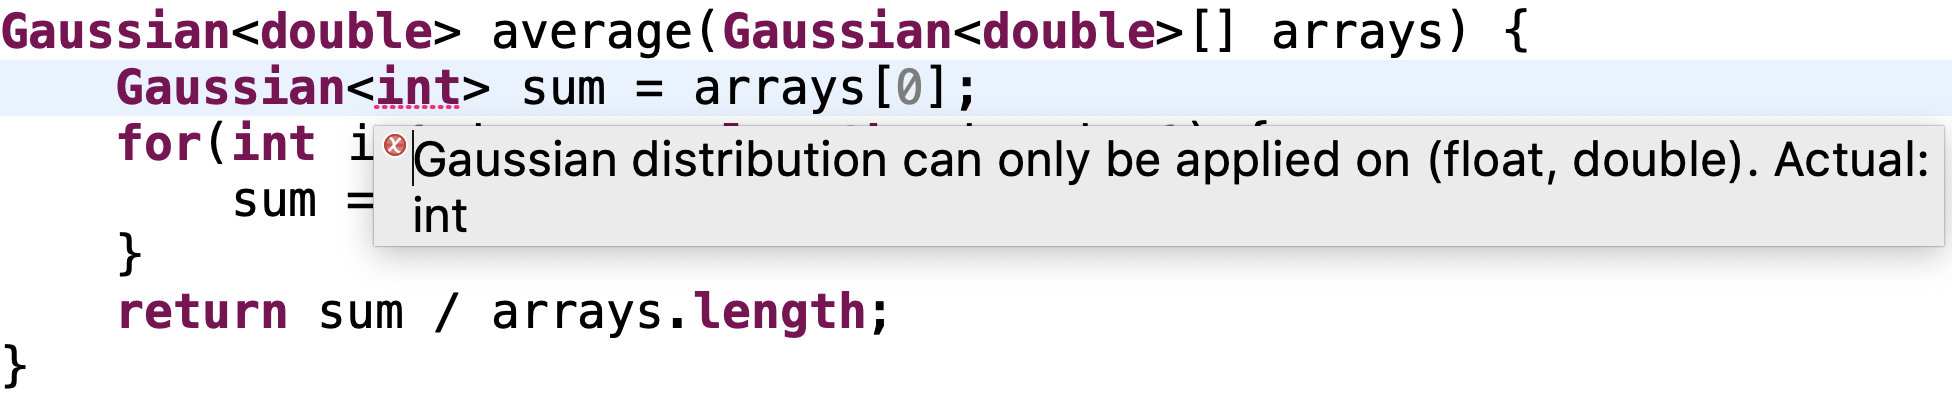
\includegraphics[width=\linewidth]{img/chapt-intro/approach/aintea-overview}
	\caption{Overview of the language proposed, \langName{}}
	\label{fig:intro:contrib:aintea}
\end{figure}

This contribution addresses the challenge of the manipulation of uncertain data (cf. Sub-Challenge \#1). 
We propose \langName{}, a language able to represent uncertain data as built-in language types along with their supported operations.
An overview of the language is depicted in~\Cref{fig:intro:contrib:aintea}.
 It contains a sampling of distributions (Gaussian, Bernoulli, binomial, Dirac delta function, and Rayleigh) that covers the different data types (booleans, numbers, and references).
 We implement a prototype of the language, publicly available on GitHub\footnote{\url{https://github.com/lmouline/aintea/}}.
 We use a real-world case study based on \gls{sg}, built with our partner Creos S.A..
It shows first that our approach does not impact the conciseness of the language.
Second, it highlights the feasibility and the advantages of uncertainty-aware type checking systems on the language level.

This contribution is under submission at the JOT Journal\footnote{\url{http://www.jot.fm/}}:
\begin{itemize}
	\item \citetitle{insubmission:2019:comlan:datauncertainty}, \citeauthor{insubmission:2019:comlan:datauncertainty}
\end{itemize}

\paragraph{A temporal knowledge \gls{metamodel}}
\begin{figure}
	\centering
	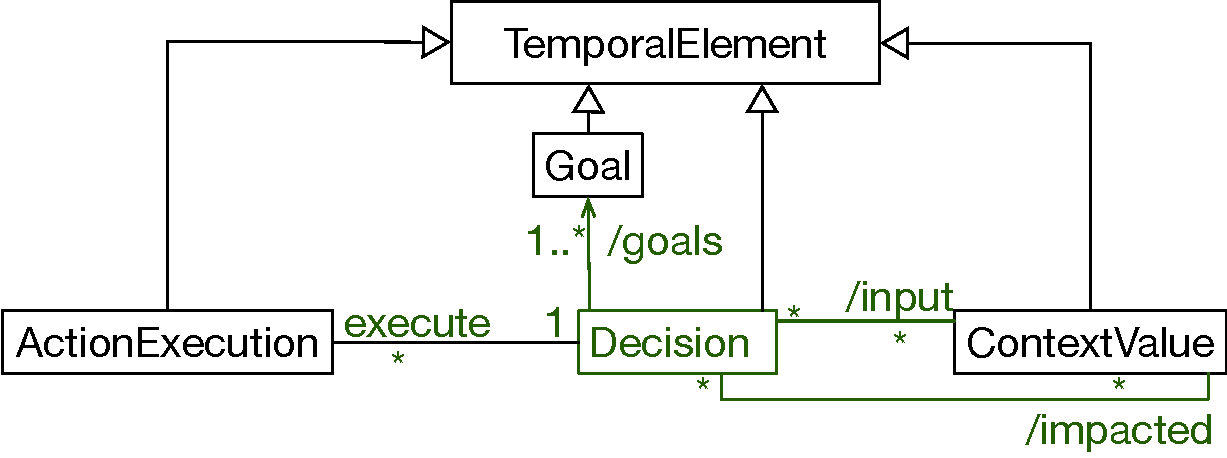
\includegraphics[width=0.6\linewidth]{img/chapt-intro/approach/tkm-overview}
	\caption{Overview of the temporal knowledge model}
	\label{fig:intro:contrib:tkm}
\end{figure}

This contribution addresses the challenge of reasoning over unfinished actions and of the understanding of \gls{adptSyst} \gls{behaviour} (cf. Sub-Challenge \#2 and \#3).
First, we formalise the common core concepts implied in adaptation processes, also referred to as \gls{knowledge}.
The formalisation is based on temporal graphs and a set of relations that trace decisions impact to circumstances.
Second, we propose a framework to structure and store the state and behaviour of a running \gls{adptSyst}, together with a high-level \gls{api} to efficiently perform diagnosis routines.
Our framework relies on a temporal model-based solution that efficiently abstracts decisions, their corresponding circumstances, and their effects.
We give an overview of the \gls{metamodel} in~\Cref{fig:intro:contrib:tkm}.
We demonstrate the applicability of our approach by applying it to a \gls{sg} based example.
We also show that our approach can be used to diagnose the behaviour of at most the last five days of a district in the Luxembourg \gls{sg} in $\sim$2.4 seconds.


Part of this contribution has been published at the IEEE International Conference on Autonomic Computing\footnote{\url{http://icac2018.informatik.uni-wuerzburg.de/}} (ICAC) and at the ACM/SIGAPP Symposium On Applied Computing\footnote{\url{http://www.sigapp.org/sac/sac2018/}} (SAC):
\begin{itemize}
	\item \citetitle{DBLP:conf/sac/MoulineB0FBMB18}, \citeauthor{DBLP:conf/sac/MoulineB0FBMB18}
	\item \citetitle{DBLP:conf/icac/MoulineBFBB18}, \citeauthor{DBLP:conf/icac/MoulineBFBB18}
\end{itemize}
\section{Structure of the document}

\begin{figure}
	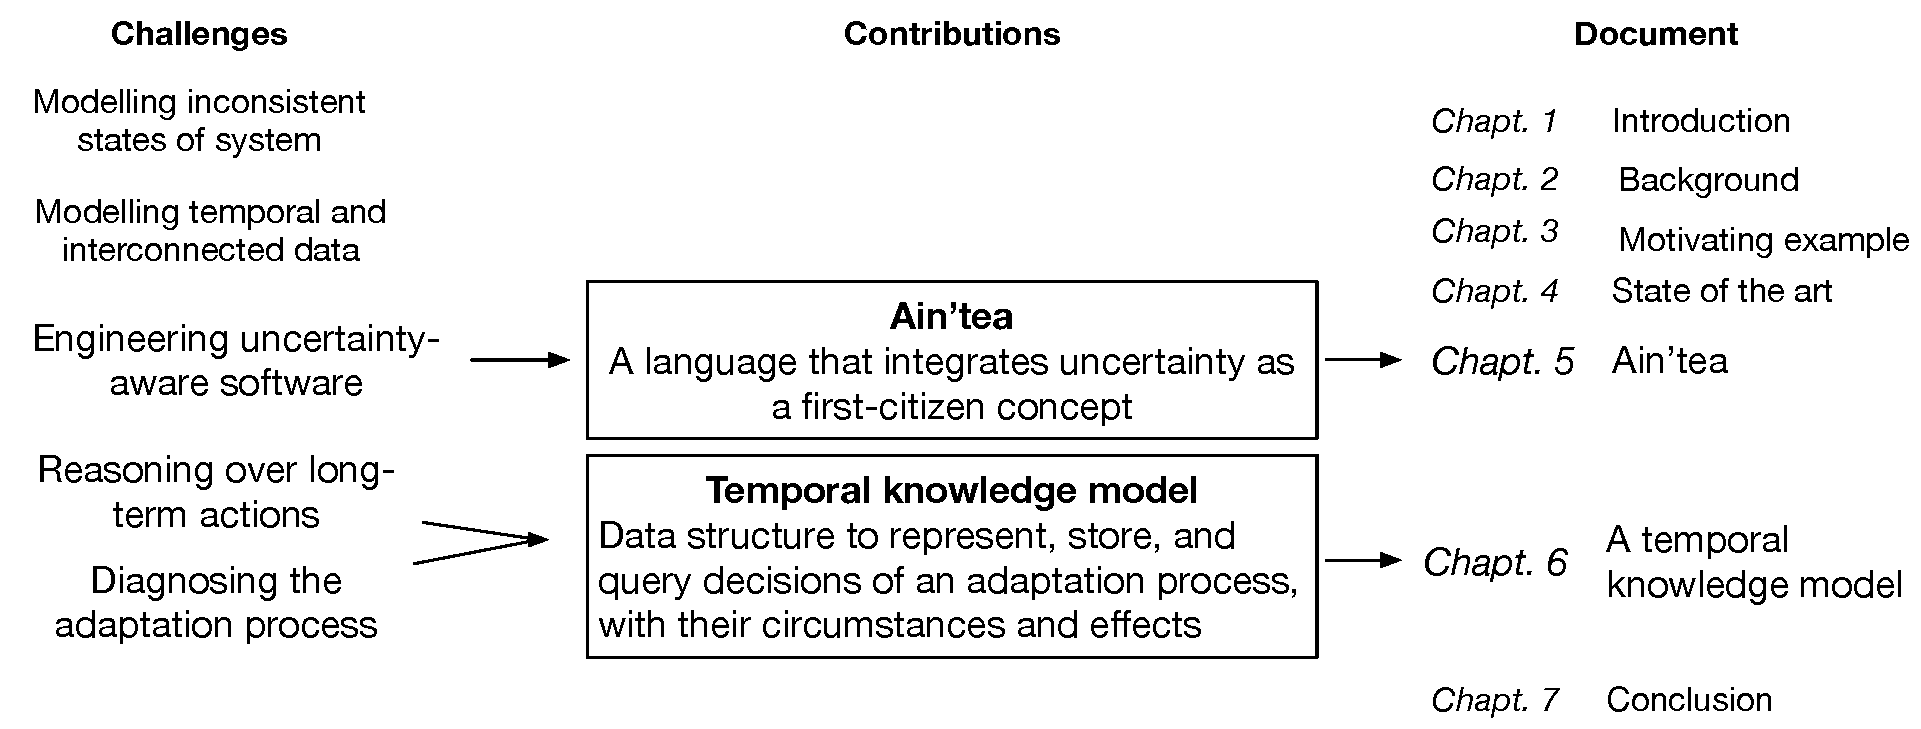
\includegraphics[width=\linewidth]{img/chapt-intro/struct/struct}
	\caption{Structure of the document}
	\label{fig:intro:structDoc}
\end{figure}

We split the remaining part of this document into six chapters, as shown in~\Cref{fig:intro:structDoc}.
First, \Cref{chapt:background} describes the necessary background of the thesis.
Then, \Cref{chapt:example} describes a motivating example, based on a \gls{sg} system.
We present concepts related to \gls{mde} and \glspl{adptSyst}.
Based on this background, we show the gap of the current state of the art in \Cref{chapt:sota}.
\Cref{chapt:aintea} and \Cref{chapt:tkm} described our two contributions.
The former details our language, \langName, that integrates uncertainty as a first-class citizen.
The latter explains our temporal \gls{metamodel} that can represent past and ongoing \glspl{action} with their circumstances and effects.
Finally, we conclude in \Cref{chapt:conclusion}, and we present a set of future works.